\subsection{Hindernisse und Bewegung}
Die Test sollen überprüfen, ob Robby ein geschlossenes Hindernis aus Wänden umrunden kann ohne Kontakt zur Wand zu verliehren und wieder am Ausgangspunkt ankommt.

\subsubsection*{Testablauf}
Robby wird in der Welt mit Blickrichtung zur Wand platziert und um ihn herum ein Hindernis, wie in Abbildung~\ref{img:obstacle} dargestellt, aufgabaut. Da die Implementierung von \mintinline{java}{void hindernisUmrunden(Runnable)} ermöglicht, Benutzeraktionen während des Umrundens durchzuführen, wird getestet, ob sich in den acht Feldern um Robby eine Wand befindet. Wenn nicht ist der Test gescheitert. Auch muss gewährleistet sein, dass er am Ende wieder an der Ausgangsposition ankommt und die Spielfläche aufgeräumt wird.

\begin{figure}
\centering
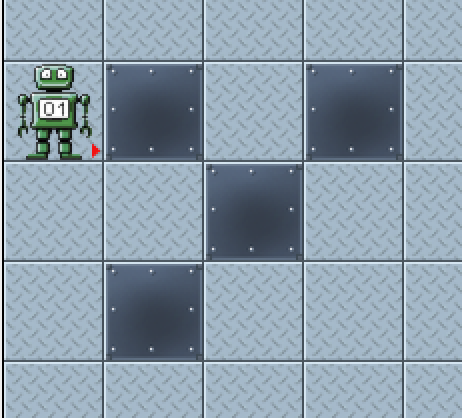
\includegraphics[width=0.8\linewidth]{img/obstacle}
\caption{Das von der Testfunktion erstellte Hindernis. }
\label{img:obstacle}
\end{figure}
